%!TEX root = ./intern_report.tex

\subsection{How I got the Opportunity}

\paragraph{}
After graduation, I wanted to continue doing higher studies and become an academic, rather than settling for a job at a company. Therefore, for my internship, I applied for research opportunities in universities and institutes around the world. I got positive response from two or three institutes, one of them being CSIRO. I sent my CV to Dr. Navinda Kottege from RAG, DATA61, CSIRO in February 2018, requesting a research internship opportunity. He asked me to complete a set of 3 timed tasks online to assess my skills in programming and algorithms. He then interviewed and offered me the position as research intern student in CSIRO for 6 months.

\paragraph{}
Initially I was informed that I am being assigned to the project titled "Computer vision based off-board autonomous UAV Navigation" under the supervision of Mr. Frederick Pauling, a highly capable and friendly senior engineer in DATA61. I was informed that knowledge in ROS (Robot Operating System) and Tensorflow would be necessary, so I spent few weeks learning the basics before the internship.

\paragraph{}
However, when I arrived at CSIRO, Mr. Frederick Pauling had been promoted into the Group Leader of RAG (Robotics and Autonomous systems Group), to lead the cutting edge robotics research in Australia. Therefore, I could not be assigned into the said project under his supervision. As a result, Uvindu and I was assigned under the supervision of Mr. Nicolas Hudson.

\paragraph{}
Mr. Nicolas Hudson arrived CSIRO only few weeks before us, after working as a senior roboticist in NASA's Jet Propulsion Laboratory, Boston Dynamics and Google's Machine Learning Division. In CSIRO he wanted to streamline the workflow of the RAG group and incorporate Machine Learning tools into their workflow seamlessly. He asked us to work with him in one of his experimental projects: "Learning Transfer Across RGB, Thermal and IR Modalities in CNNs". After about a week, Uvindu requested for a project that is more focused on hardware. Hence, he asked us to modify Trailnet for autonomous indoor navigation.

\newpage
\subsection{Trailnet: A Classification Network for Autonomous Trail Navigation}

\subsubsection{Trailnet: An Introduction}

In 2017, four researchers published a paper titled "Toward Low-Flying Autonomous MAV Trail Navigation using Deep Neural Networks for Environmental Awareness"~\cite{trailNet} (Trailnet paper in short) with the funding of NVIDIA. The paper describes the following:

\begin{itemize}
    \item Merits of approaching autonomous navigation as a classification problem
    \item Architecture of their Trailnet CNN, a modified version of Resnet-18. ~\cite{resnet}
    \item Data collection techniques for the Trailnet CNN
    \item Training Trailnet with a relatively small dataset
    \item Hardware hierarchy and the command flow between cameras, NVIDIA Jetson TX2 ~\cite{jetson_tx2} running ROS and the flight control board.
    \item Usage of YOLO for obstacle detection and algorithm for obstacle avoidance.
    \item Results and observations after flying the quadcopter autonomously in the forest trail for several kilometers.
\end{itemize}


\newpage
\subsection{Building Wallie: A Hardware Platform for Data Collection and Deployment}

\begin{figure}[H]
    \centering
    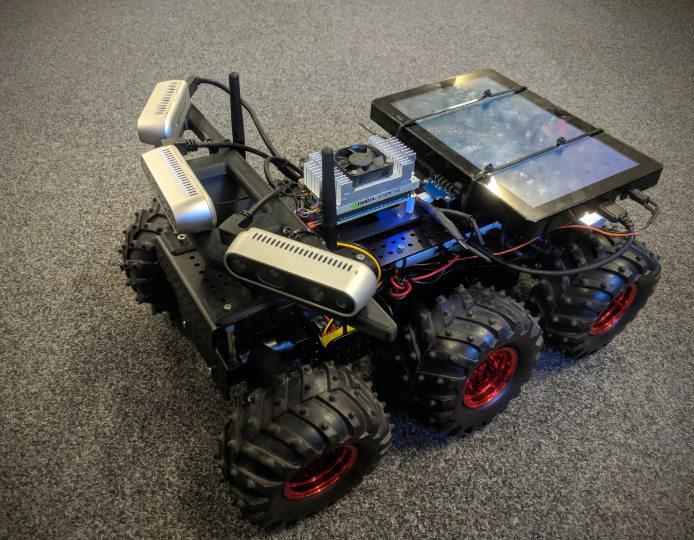
\includegraphics
        [width=10cm]
        {figures/wallie.PNG}
    \caption{Wallie: The Robot \label{Fig:wallie}}\vspace{-4mm}
\end{figure}

\begin{figure}[H]
    \centering
    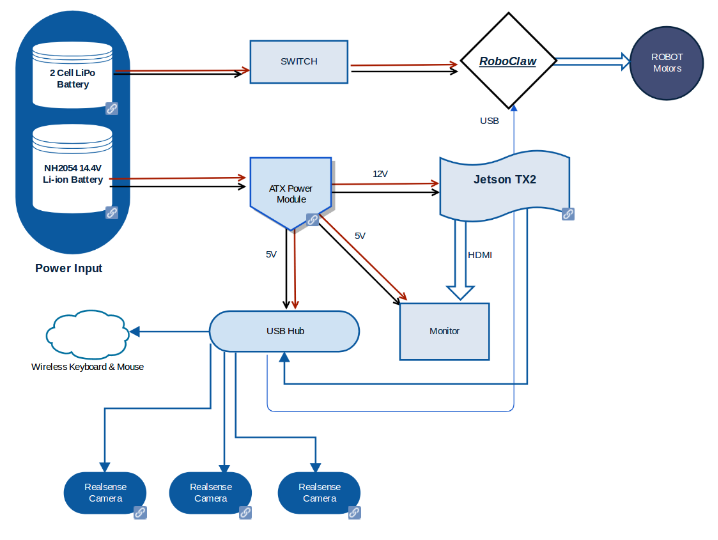
\includegraphics
        [width=10cm]
        {figures/wallie_hardware.PNG}
    \caption{Wallie: Hardware Hierarchy }\vspace{-4mm}
\end{figure}


\subsubsection*{NVIDIA Jetson TX2}

\begin{figure}[H]
    \centering
    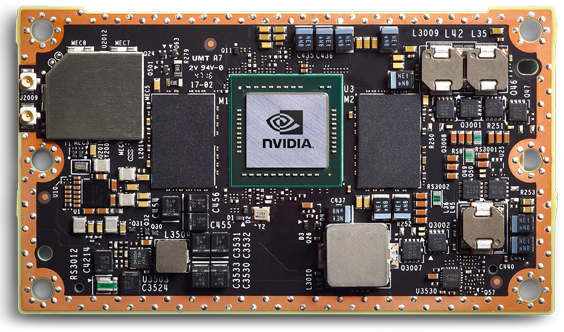
\includegraphics
        [width=8cm]
        {figures/jetson.png}
    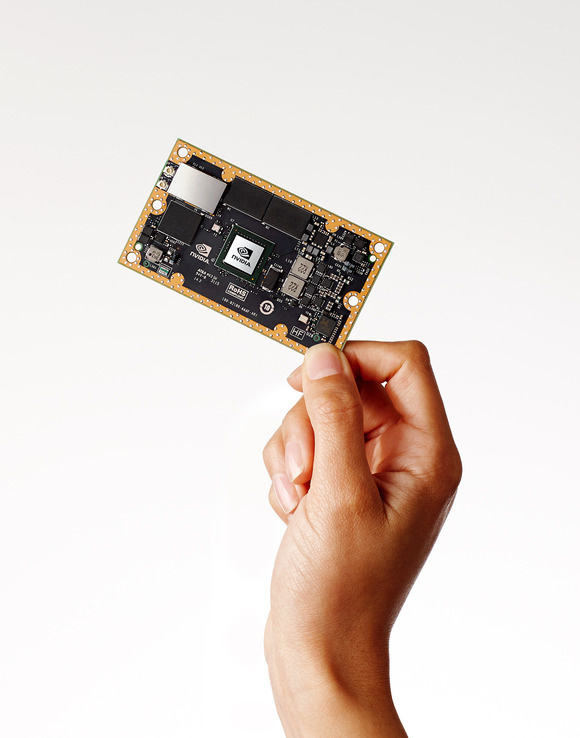
\includegraphics
        [height=5cm]
        {figures/jetson_scale.jpg}
    \caption{NVIDIA Jetson TX2 }\vspace{-4mm}
\end{figure}



\subsubsection*{Intel Realsense Depth Camera D435}

\begin{figure}[H]
    \centering
    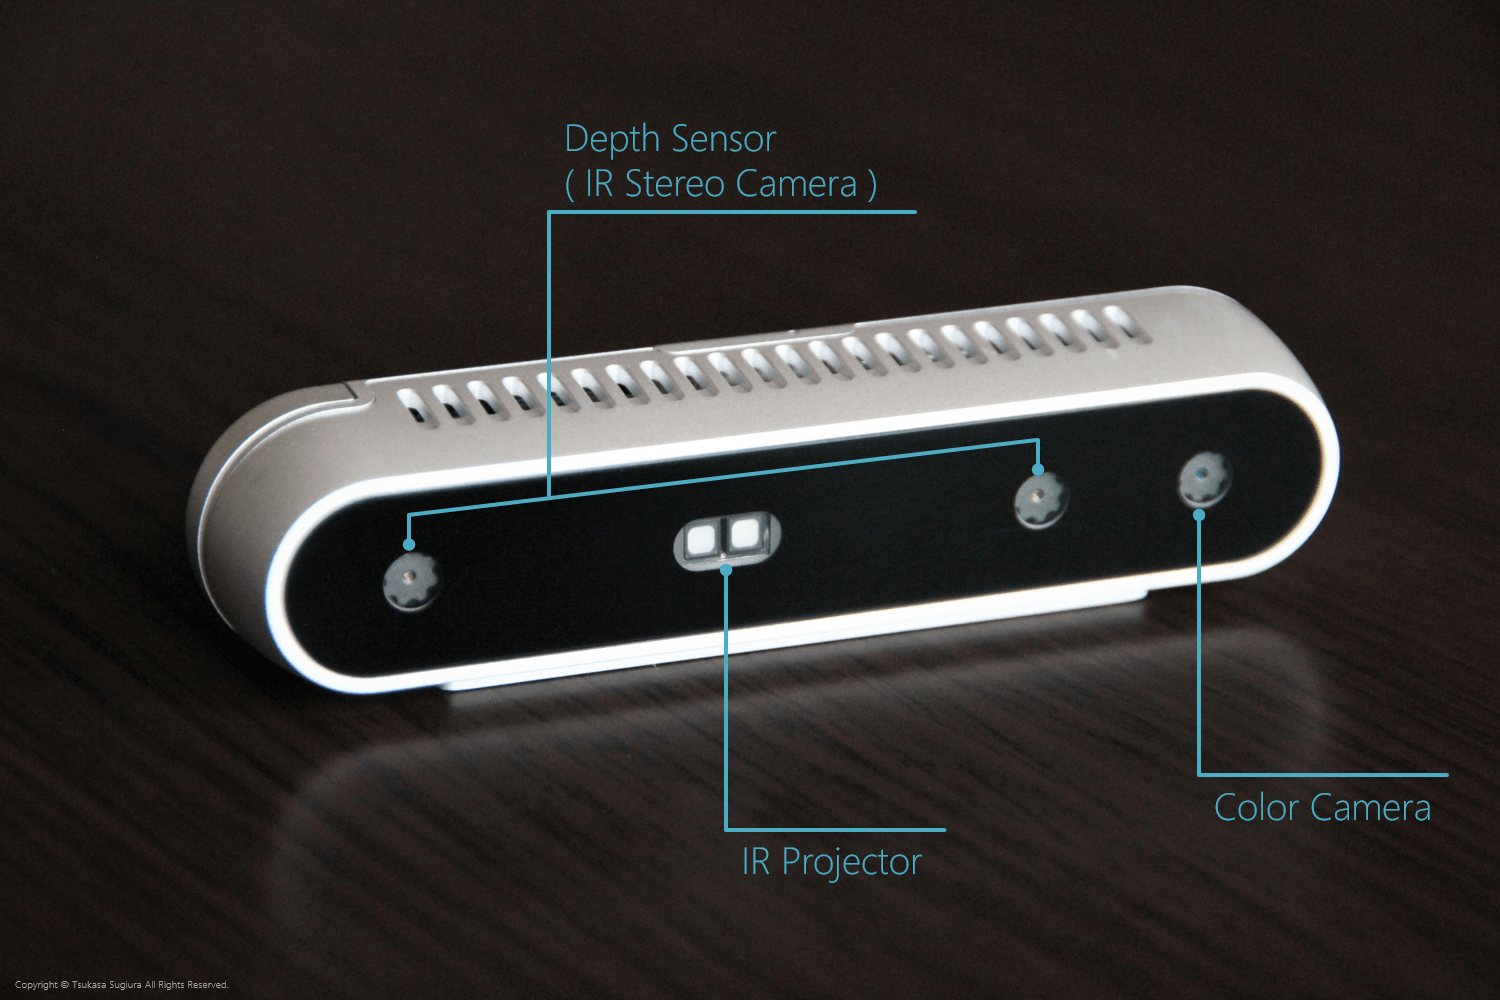
\includegraphics
        [width=12cm]
        {figures/realsense.png}
    \caption{Intel Realsense D435}\vspace{-4mm}
\end{figure}

\subsubsection*{Roboclaw Motor Controller}

\begin{figure}
    \centering
    \begin{minipage}{.5\textwidth}
        \centering
        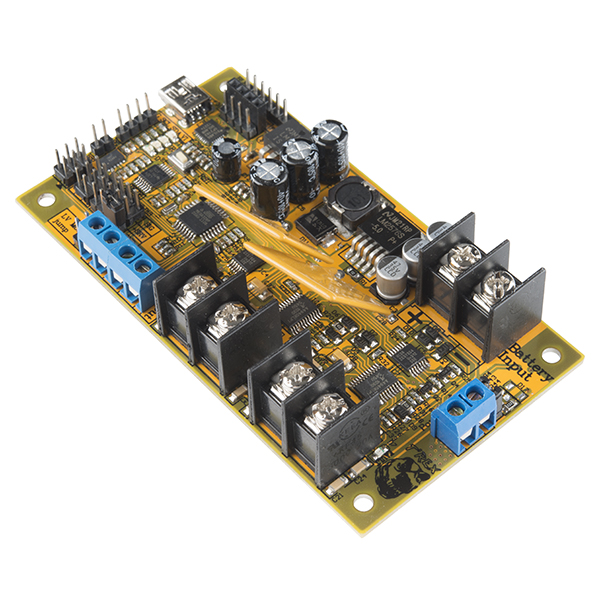
\includegraphics[width=\linewidth]{figures/trex.jpg}
        \captionof{figure}{TREX Motor Controller}
        \label{fig:test1}
    \end{minipage}%
    \begin{minipage}{.5\textwidth}
        \centering
        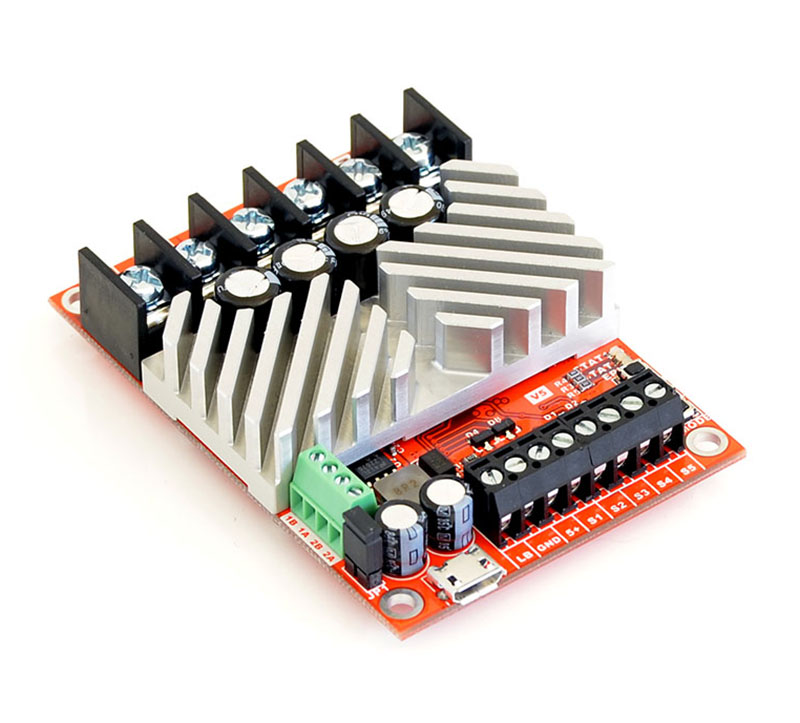
\includegraphics[width=\linewidth]{figures/roboclaw.jpg}
        \captionof{figure}{Roboclaw Motor Controller}
        \label{fig:test1}
    \end{minipage}
\end{figure}



\subsubsection*{Problems Faced and Solutions}





\newpage
\subsection{Designing and Implementing an Efficient End-toEnd Pipeline for Machine Learning in Robotics}

\begin{figure}[H]
    \centering
    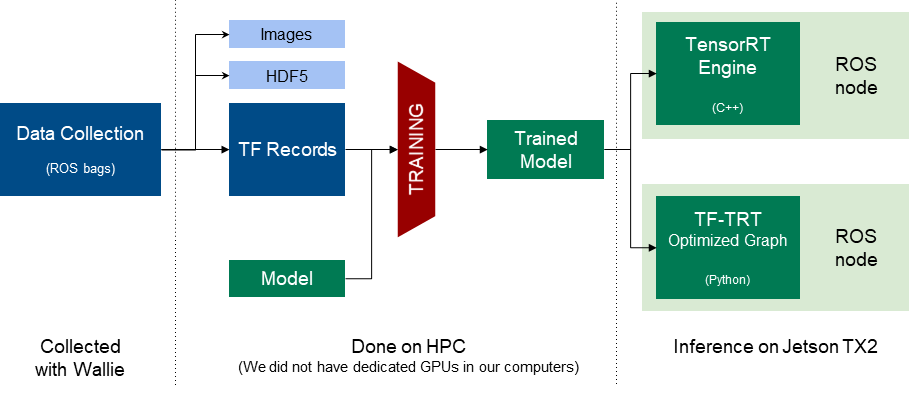
\includegraphics
        [width=16cm]
        {figures/full_pipeline.PNG}
    \caption{End-to-End Pipeline \label{Fig:pipeline}}\vspace{-4mm}
\end{figure}

\subsubsection{Training on Supercomputers}

\subsubsection{TF Records}

\begin{figure}[H]
    \centering
    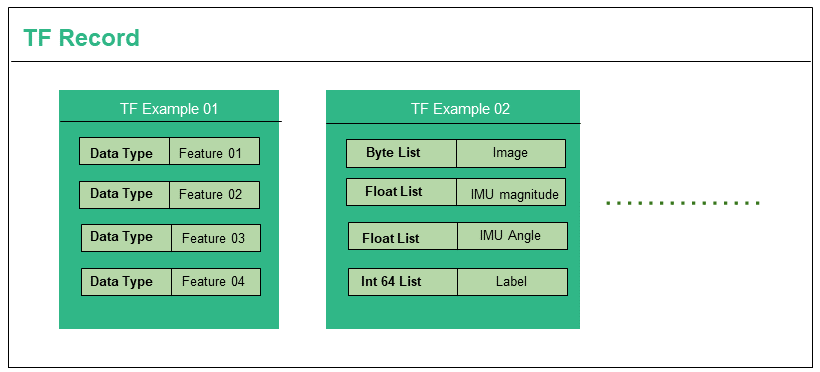
\includegraphics
        [width=9cm]
        {figures/tfrecord_structure.PNG}
    \caption{Structure of a TF Record}\vspace{-4mm}
\end{figure}

\subsubsection{TensorRT: Deployment on a low power device}

\begin{figure}[H]
    \centering
    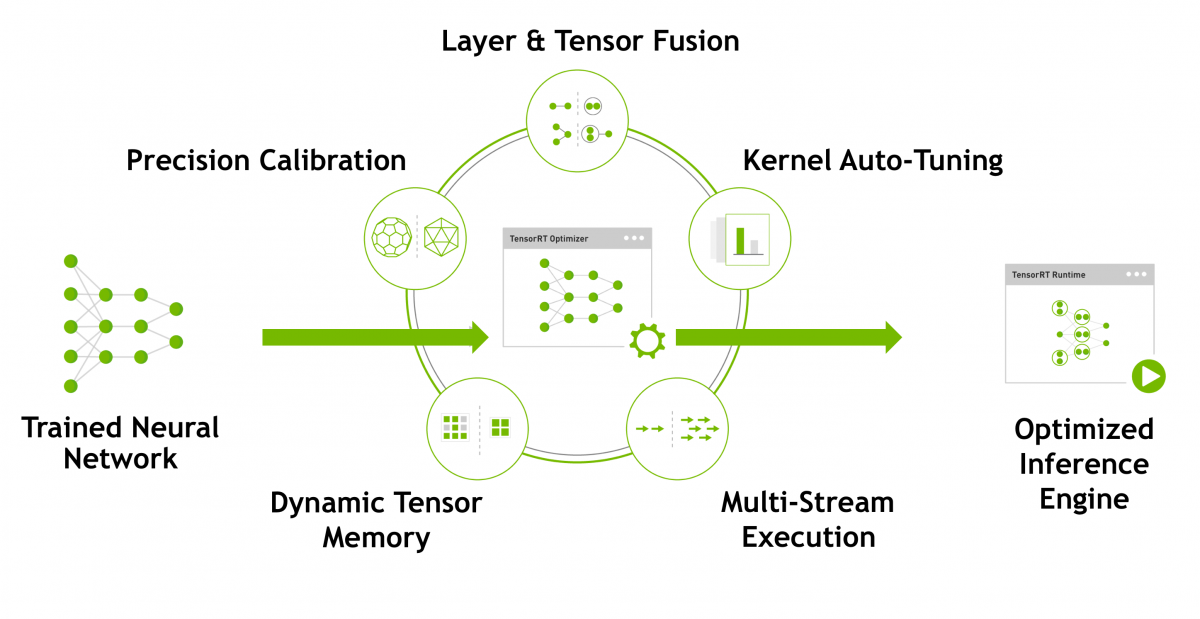
\includegraphics
        [width=13cm]
        {figures/trt.png}
    \caption{TensorRT in a nutshell}\vspace{-4mm}
\end{figure}

\begin{figure}[H]
    \centering
    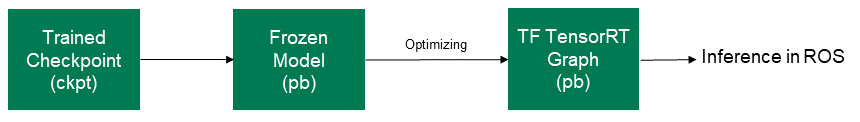
\includegraphics
        [width=13cm]
        {figures/deploy_pipeline_cpp.PNG}
    \caption{Deployment Pipeline: C++}\vspace{-4mm}
\end{figure}

\begin{figure}[H]
    \centering
    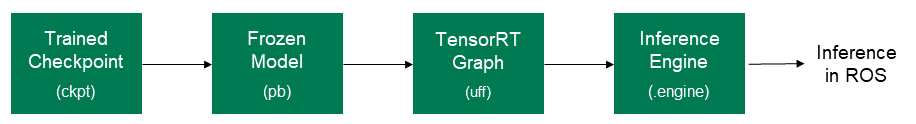
\includegraphics
        [width=13cm]
        {figures/deploy_pipeline_python.PNG}
    \caption{Deployment Pipeline: Python}\vspace{-4mm}
\end{figure}

\subsubsection{Problems Faced and Solutions}



\newpage
\subsection{Hillnet: An Experimental Attempt at Utilizing ML for Hill Climbing}

\subsubsection{Preprocessing IMU and Velocity Data}

\subsubsection{Classification Approach}

\subsubsection{Regression Approach}

\subsubsection{Merging Scaler and Image Inputs}

\subsubsection{Problems Faced and Solutions}



\newpage
\subsection{Life at CSIRO}
    

\subsubsection{Reading Groups and DATA61 Meetings}

\subsubsection{DATA61 Live Event}

\begin{figure}[H]
    \centering
    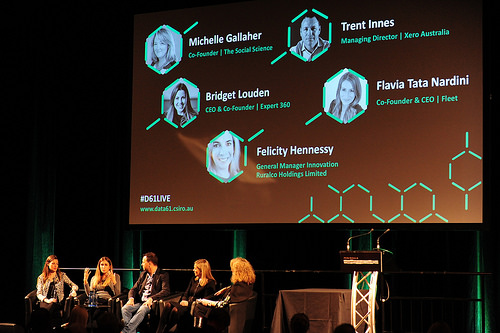
\includegraphics
        [height=5cm]
        {figures/data61_live_1.jpg}
    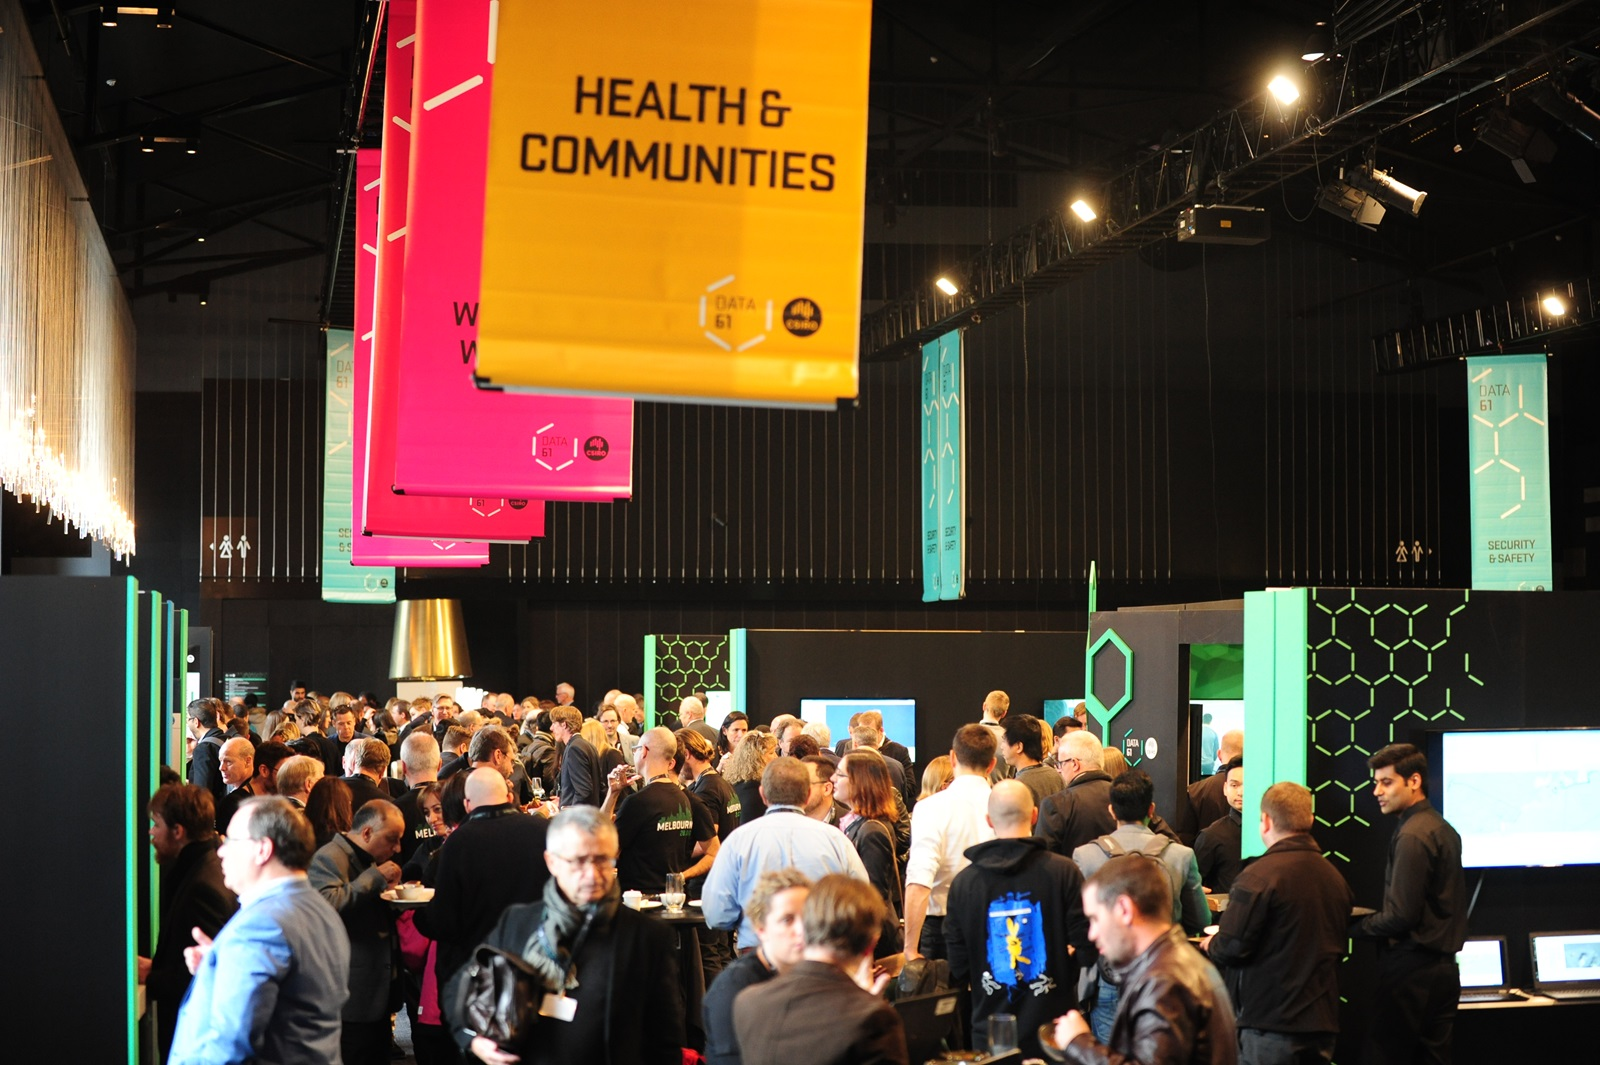
\includegraphics
        [height=5cm]
        {figures/data61_live_2.jpg}
    \caption{DATA61 LIVE Event}\vspace{-4mm}
\end{figure}


\newpage
\subsection{Presenting the Pipeline at Reading Group to the Scientists}

